\section{Hardware}
In diesem Kapitel wird die Hardware der Steuerung im Detail erläutert. Es wird genauer auf die technischen Details der verwendeten Komponente eingegangen und auf ihre Aufgabe in der Steuerung.

% \begin{itemize}
%     \item Beschreibung, Zweck der TECs
%     \item Beschreibung der TECs und wo diese platziert sind mit Illustrationen
% \end{itemize}

\subsection{Raspberry PI}
Dieser wurde ausgewählt, weil dieser mit sämtlichen industriellen Schnittstellen kompatibel ist. Darunter auch mit der SPS, die im nächsten Kapitel beschrieben ist. Dieser ist die Hauptkomponente und dient als Zentrale für die Evaluierung sämtliche Berechnungen und gibt die Befehle an den TEC-Treiber und an den Diodetreiber und steuert die Digitalanzeige. Der Rechner ist direkt auf der SPS montierbar und benötigt somit weniger Platz im Gehäuse der Steuerung. Die Kommunikation des Rechners zur SPS erfolgt über ein Flachbandkabel. Worüber mit Pythonprogrammen direkt Aus- und Eingänge auf der SPS angesteuert werden können. Somit ist es möglich etliche weitere Komponente anzuschliessen und zu steuern. So auch der Diodentreiber, der im Kapitel \ref{chptr:_diodentreiber} näher beschrieben wird. Der TEC-Treiber kommuniziert direkt über die USB Schnittstelle auf dem Rechner und muss nicht über die SPS gesteuert werden.\\
Das Betriebssystem des Raspberry PI ist ein Derivat des Linux Betriebssystems. Mit einem Image speziell für einen Raspberry PI, können standardmässig Programme zum Programmieren von Pythonskripten und die Pythoninstallation mit installiert werden. Die weiter oben beschriebenen Standardbibliotheken sind ebenfalls im der Basisinstallation der Pythondistribution enthalten. Die zusätzlichen Bibliotheken von Drittanbietern müssen jedoch noch nach installiert werden. Diese sind im Anhang beschrieben.
% Dieser hat eine Arbeitsspannung von 5V.

\begin{figure}[H]
    \centering
    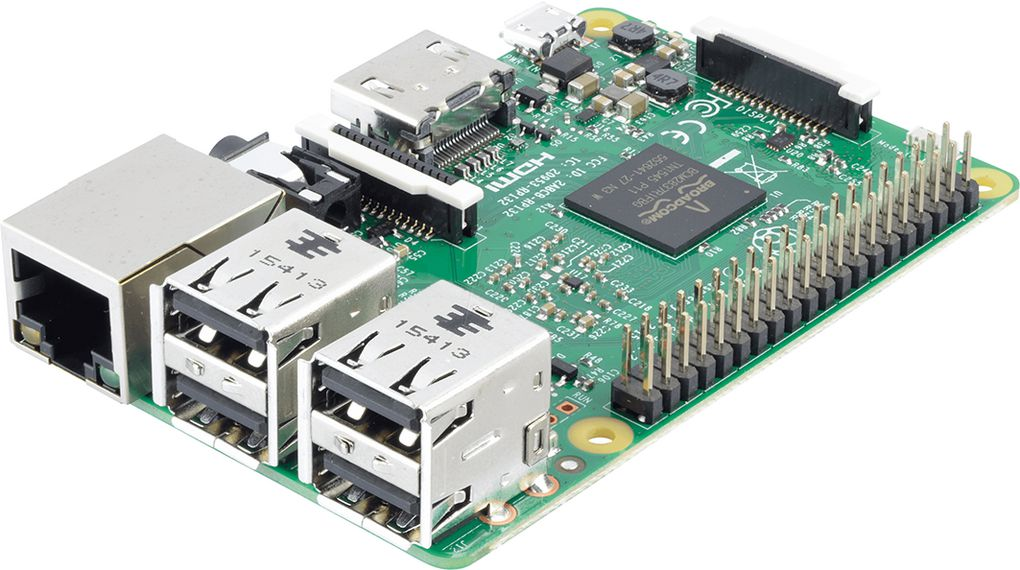
\includegraphics[scale=0.25]{98_images/raspberry_pi_version_3_b.jpg}
    \caption{Ein \textit{Raspberry PI}-Einplatinenrechner der Version  3B+.}
    \label{fig:raspberry_pi_3b+}
\end{figure}

\subsection{SPS - PiXtend}
Die Aus- und Eingänge, die der Raspberry PI Steuert sind mit einer SPS des Herstellers PiXtend L 2.1 realisiert. Dies ist eine Steuerung, auf welche der Rechner direkt aufgeschraubt werden kann. Alle benötigten Ein- und Ausgänge für die Steuerung des Pumpdiodentreibers befinden sich direkt auf der Steuerung. Von grosser Wichtigkeit sind die analogen Ein- und Ausgänge um den Ausgangsstrom des Treibers zu steuern bzw. den Ausgangsstrom zurück in die SPS zu geben, um später die optische Leistung zu evaluieren. Die Fähigkeit analoge Signale zu verarbeiten ist der Grund diese Steuerung auszuwählen.
% Daneben erfüllt diese SPS alle Voraussetzungen, damit der Raspberry PI einwandfrei läuft. 

\begin{figure}[H]
    \centering
    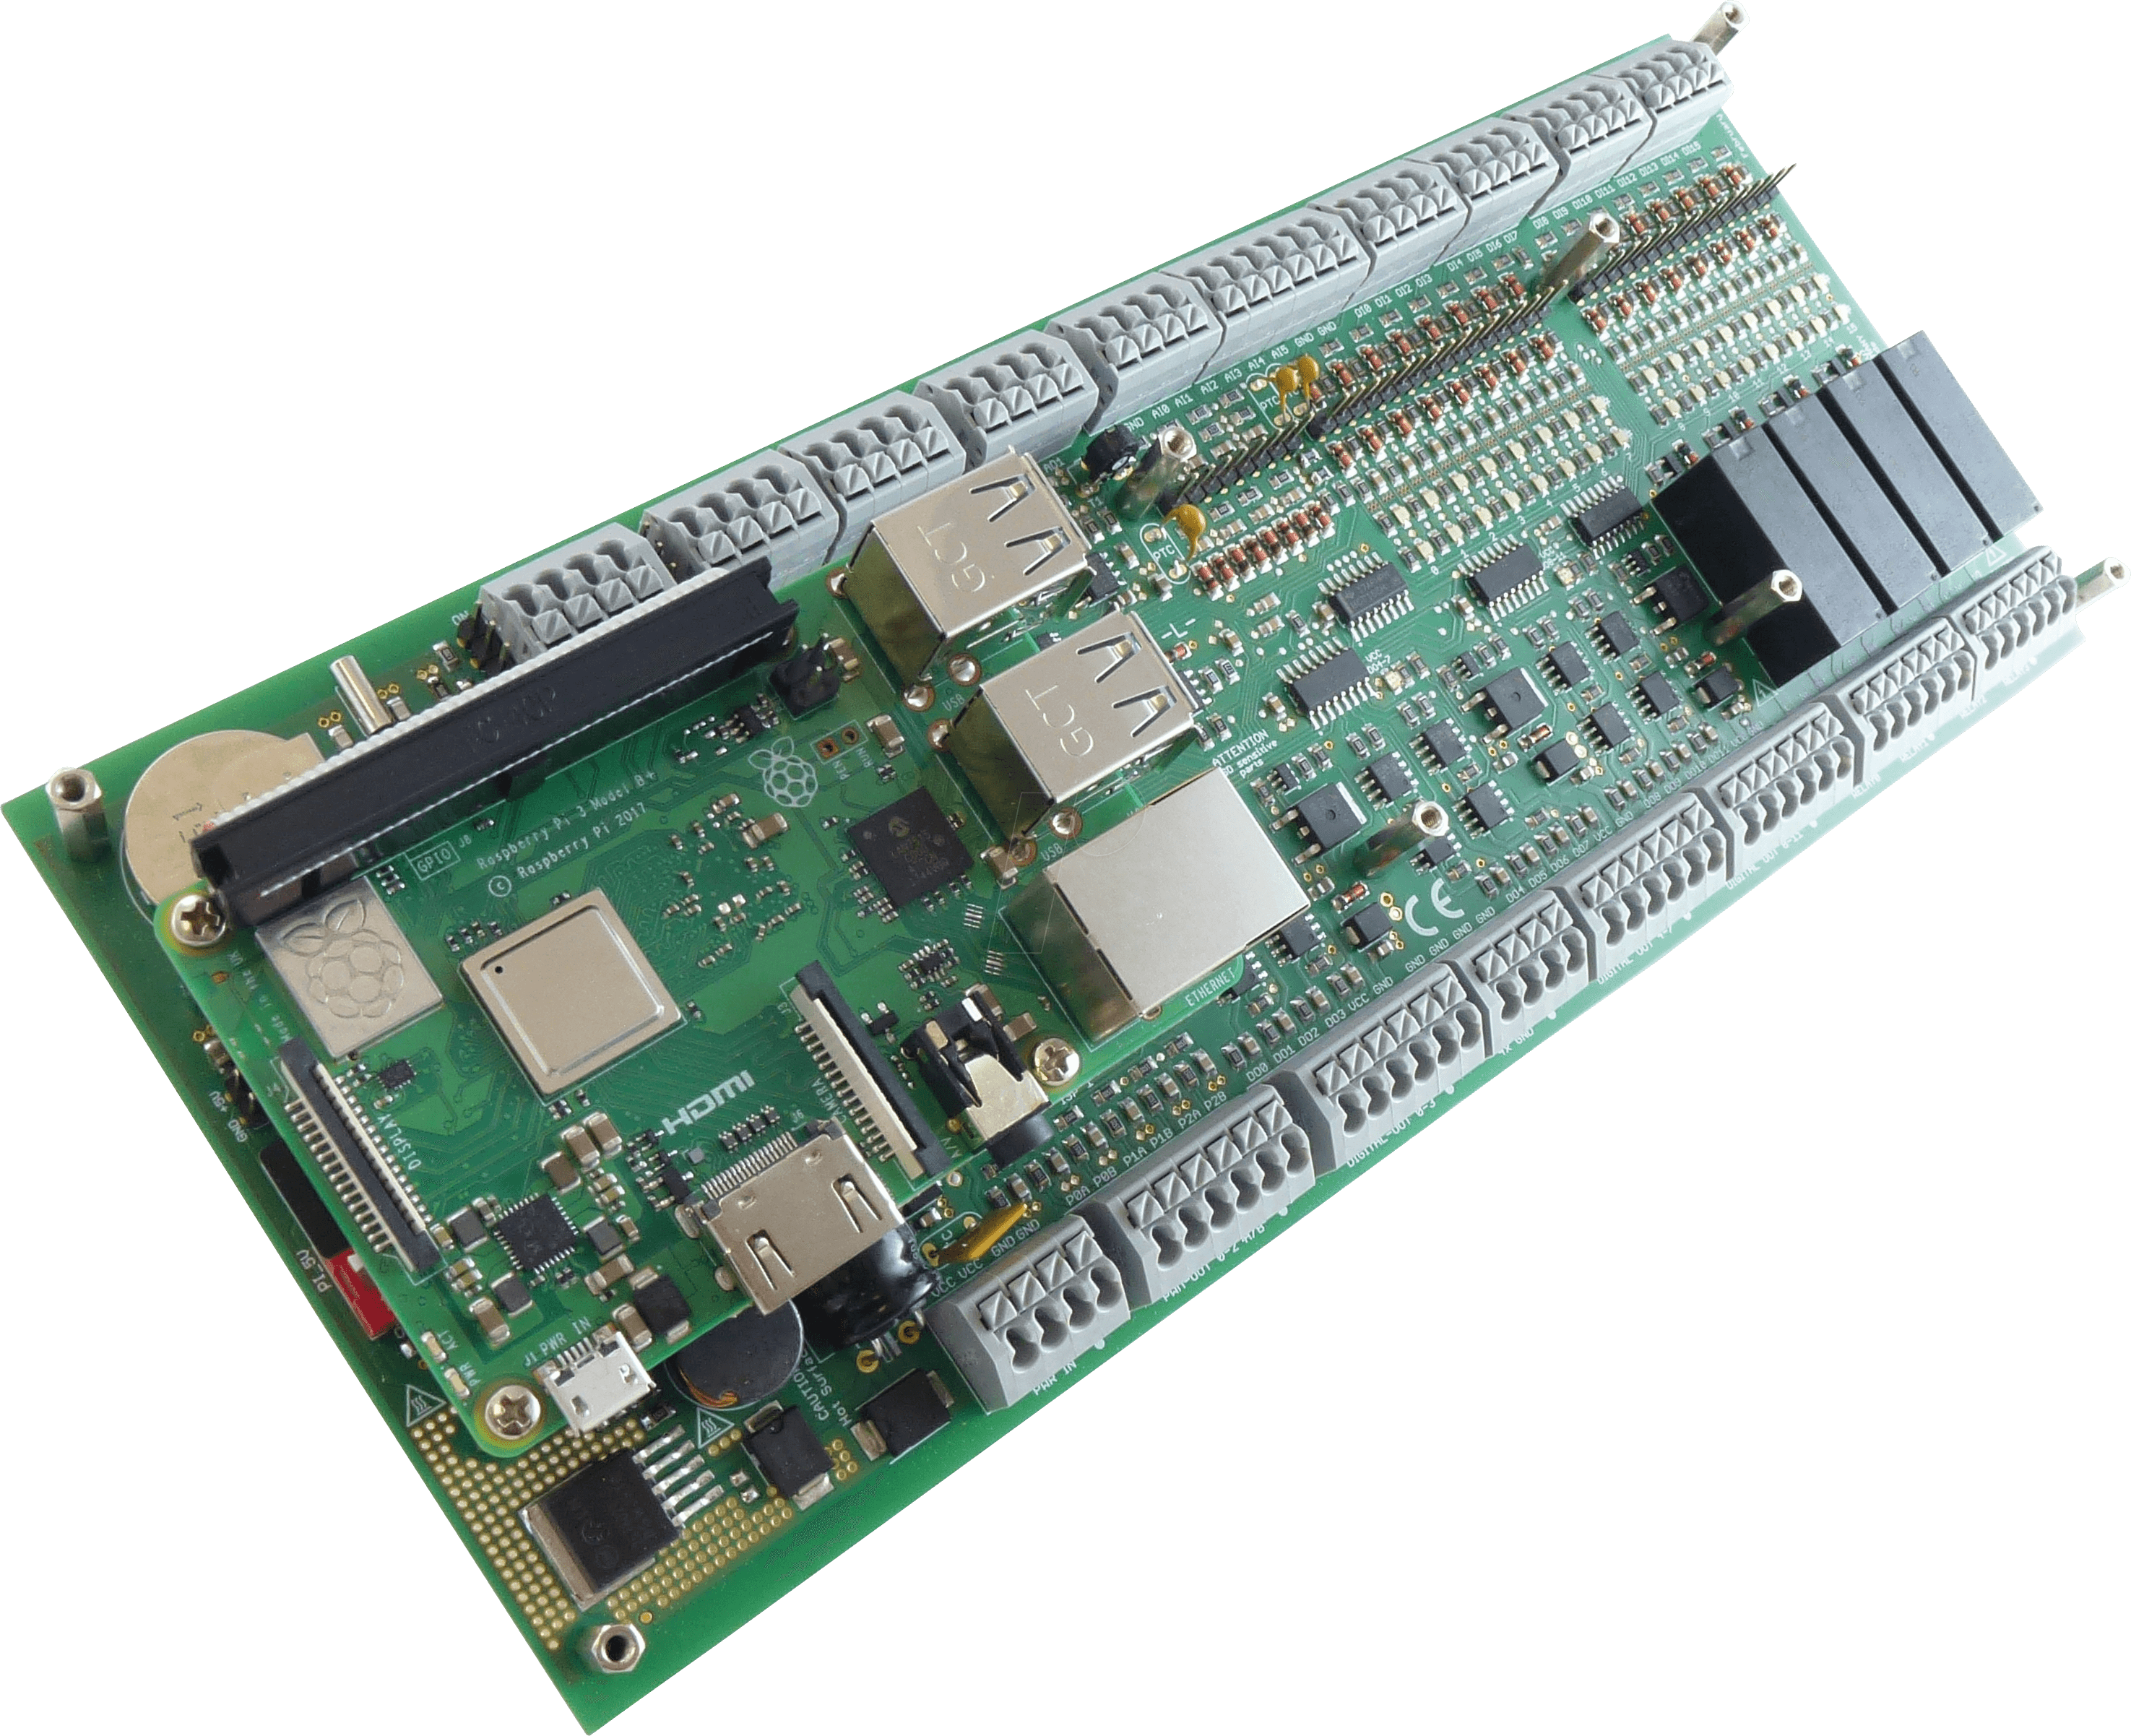
\includegraphics[scale=0.08]{98_images/pixtend_l_basic.png}
    \caption{Die \textit{SPS PiXtend L V2.1} vom Hersteller \textit{Kontron}.}
    \label{fig:sps_pixtend_hw}
\end{figure}

\subsection{Thermoelektrischer Kühler - TEC}
Die beiden verwendeten TECs werden unter der Pumpdiode bzw. und der Halterung des Alexandritkristalls montiert. Sie dienen dazu die Wärme vom Kristall und von der Pumpdiode ableiten. Werden die Temperaturen an den zu kühlenden bzw. zu heizenden Objekten mit Sensoren gemessen, kann eine optimale Temperatur eingestellt werden. Dieser befindet sich direkt unter der Halterung des Kristalls. Für den Kristall befindet sich die optimale Temperatur im Bereich von 18°C.

% \begin{figure}[H]
%     \centering
%     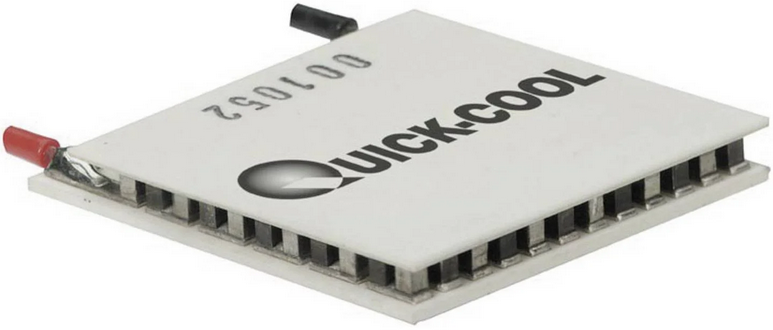
\includegraphics[scale=0.7]{98_images/peltier_modul.PNG}
%     \caption{Abgebildet ist ein thermoelektrischer Kühler.}
%     \label{fig:tec_free_hw}
% \end{figure}

\begin{figure}
    \centering
    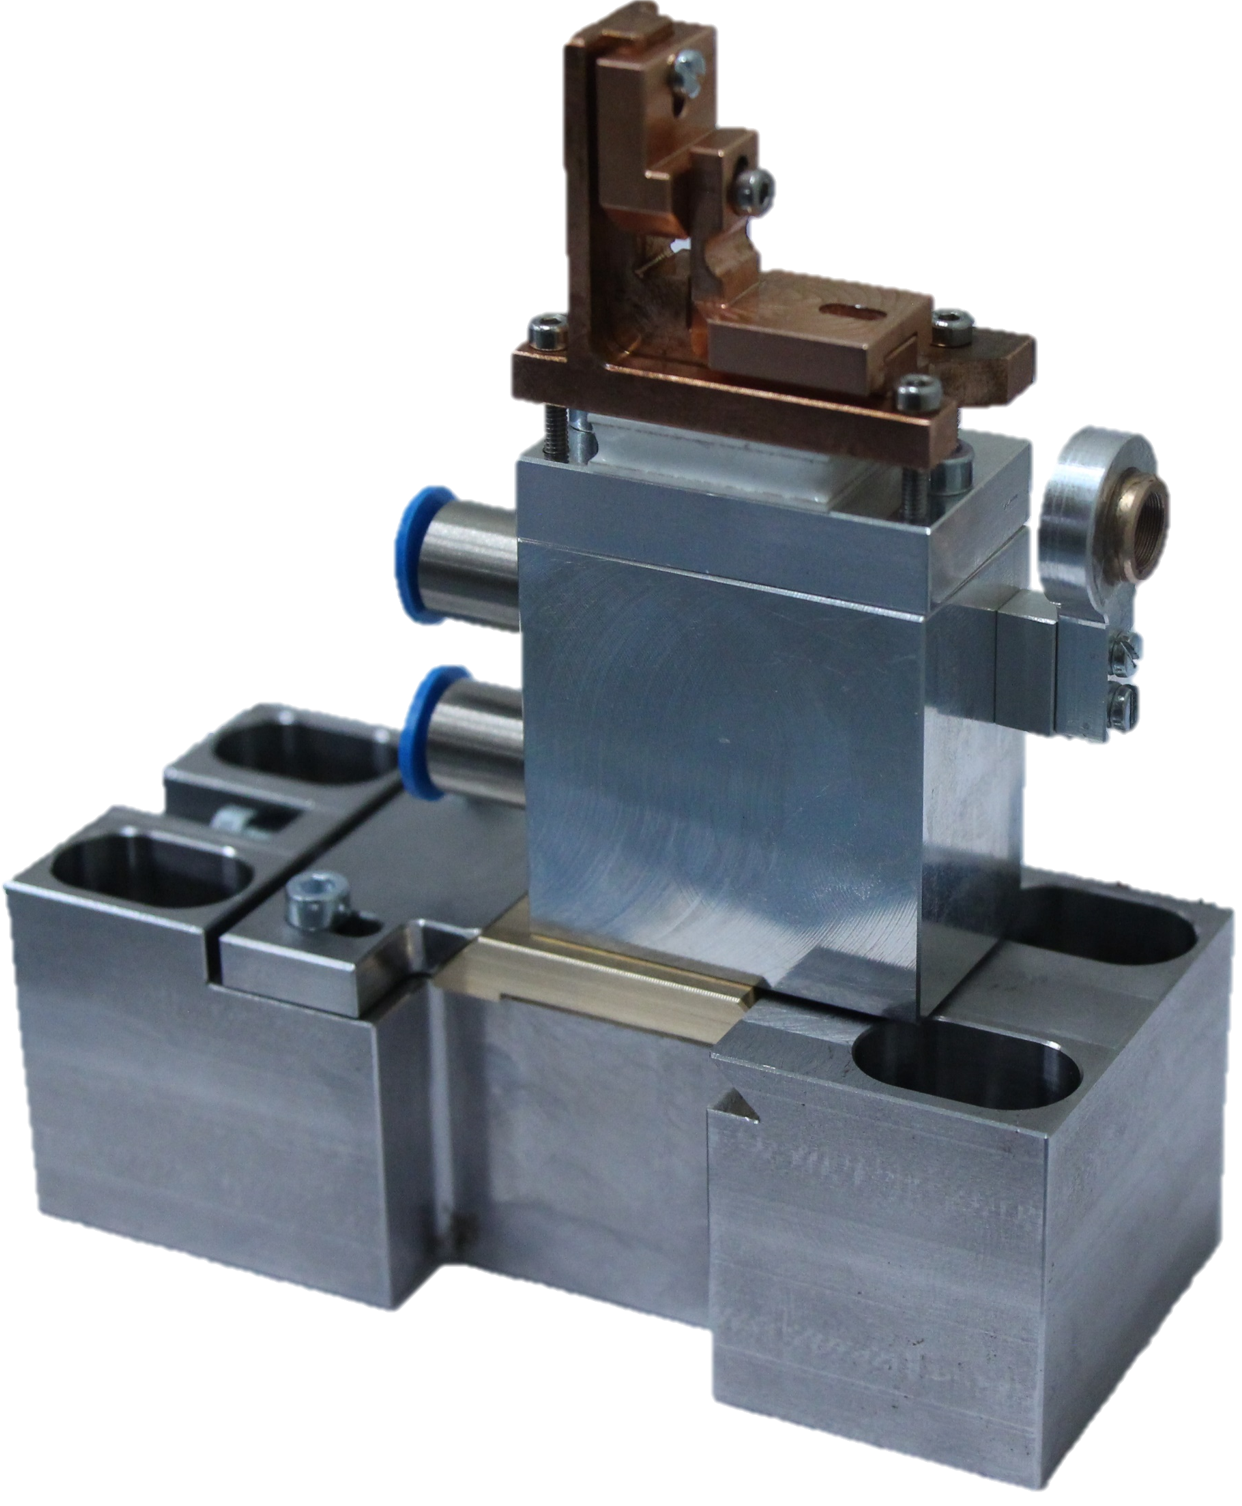
\includegraphics[scale=0.3]{98_images/real_front_02.PNG}
    \caption{In der Abbildung ist der TEC in der Kristallhalterung gezeigt.}
    \label{fig:tec_cr_hw}
\end{figure}

\begin{figure}
    \centering
    % \includegraphics{}
    \caption{Abgebildet ist der thermoelektrische Kühler für die Diode. Gleich wie beim Alexandritkristall befindet sich dieser direkt unter der Diode. Für eine bessere Wärmeleitung wird einen Wärmeleitpaste auf die Flächen des TECs aufgetragen. Der ideale Temperaturbereich für die Diode ist um die 20°C.}
    \label{fig:tec_di_hw}
\end{figure}

\subsection{TEC-Treiber}
\label{label_tec_treiber}
Aus dem Grund, dass zwei TECs gesteuert werden sollen, wurde ein zwei-kanaliger TEC-Treiber des Herstellers Meerstetter Engineering verwendet, dieser erfüllt alle Forderungen. Obwohl die Leistung von diesem zu hoch ist, wurde dieser ausgewählt. Dieser war bereits im Institut vorhanden.\\
Auf der Softwareseite sind die Signale, hier die Temperaturen, eindeutig identifizierbar, was mit zwei ein-kanaligen Treibern nicht ohne Weiteres möglich gewesen wäre. Die Informationen werden über einen BUS an den Rechner gesendet und da weiter verarbeitet bzw. verwendet.
Die Temperaturen der TECs werden über einen PID-Regler eingestellt. Der Treiber von Meerstetter Engineering ist in der Lage diese PID-Parameter automatisch zu finden und müssen nicht gesucht oder gar separat berechnet werden. Die TECs können lediglich eine maximale Leistung aufnehmen, aus Sicherheitsgründen muss der Strom deshalb begrenzt werden. Bei Zerstörung der TECs könnte auch die Pumpdiode und auch der Kristall in Mitleidenschaft gezogen werden.\\

\begin{figure}[H]
    \centering
    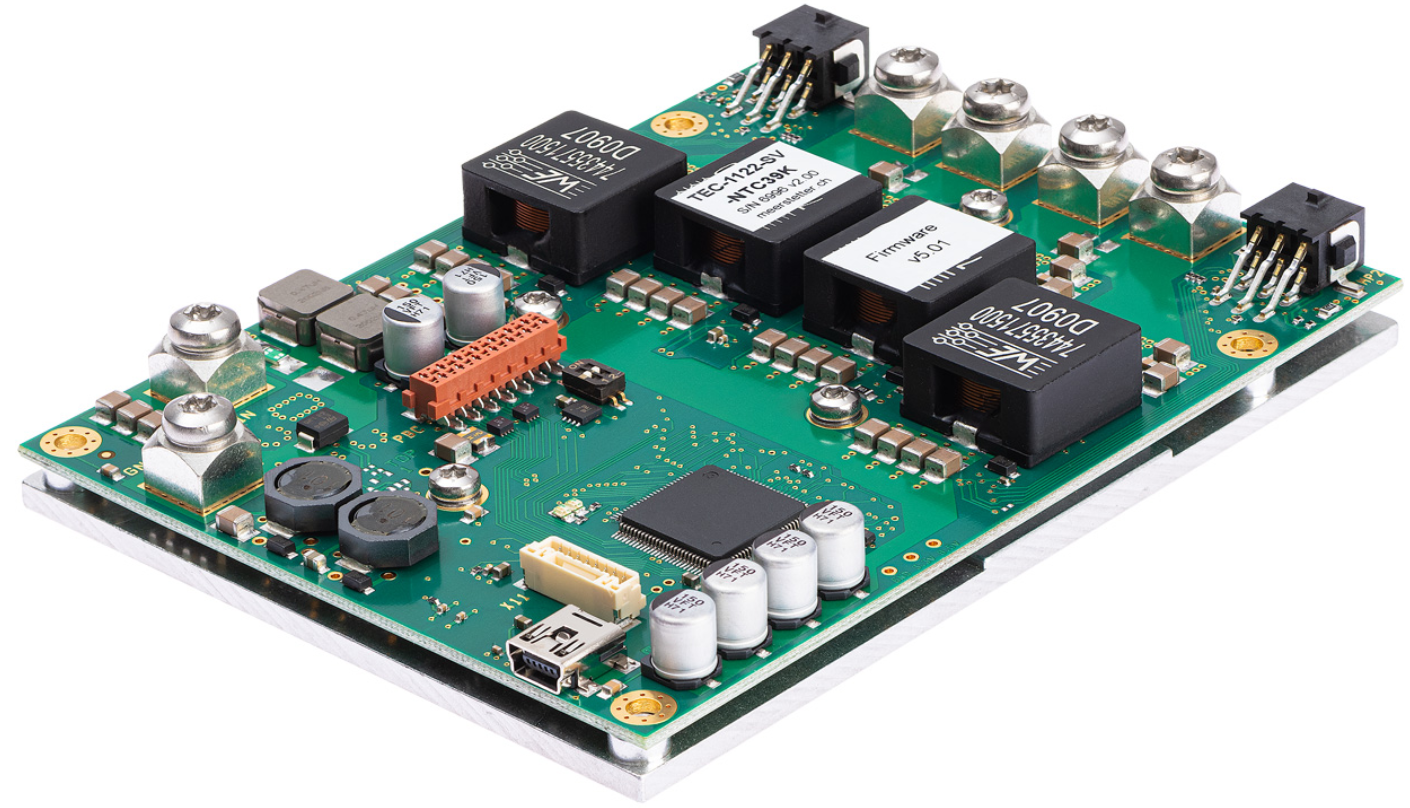
\includegraphics[scale=0.2]{98_images/tec_controller_real_isometry_meerstetter.PNG}
    \caption{Ein zwei-kanaliger TEC-Treiber vom Hersteller Meerstetter Engineering.}
    \label{fig:tec_treiber_hw}
\end{figure}

\subsection{Pumpdiodentreiber}
\label{chptr:_diodentreiber}
Der Pumpdiodentreiber oder auch Diodentreiber wurde vom Hersteller \textit{OptLaser} bezogen. Auf der Abb. \ref{fig:diodentreiber_hw} sind die Eingänge für die Energieversorgung zu sehen und daneben die analogen bzw. PWM-Eingänge zum steuern des Ausgangstroms. Die Pumpdiode wird mit 30V und bis zu 0.5A betrieben, benötigt dem entsprechend eine Eingangsleistung von mindestens 15W. [5] Der Diodentreiber verfügt über eine Spannung von 30V und kann bis zu 1.5A speisen. Um die Laserdiode jedoch vor der Zerstörung zu bewahren wurde die Stromstärke auf 0.8A beschränkt dies wurde in der Software so hinterlegt. Auf den Aufbau der Software des Diodentreibers wird im Kapitel \ref{chptr:software} genauer eingegangen.

\begin{figure}[H]
    \centering
    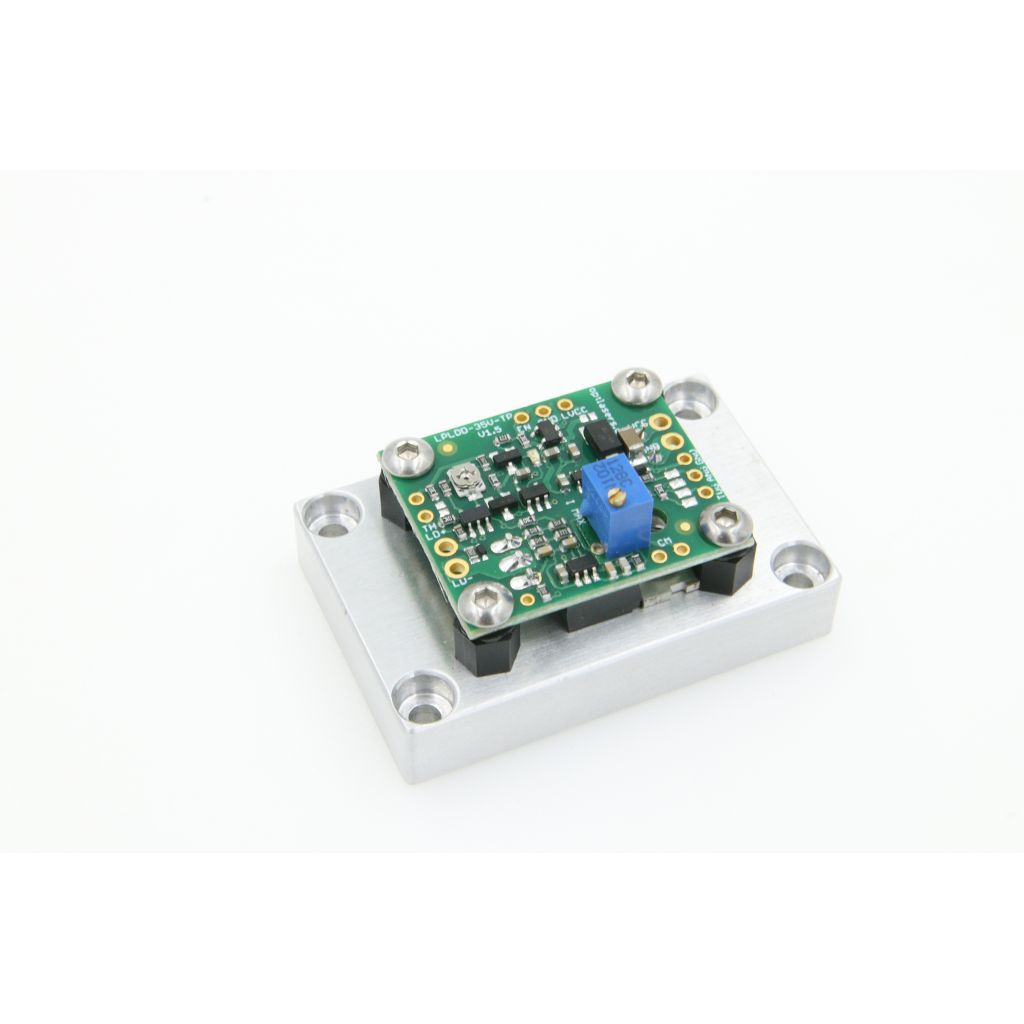
\includegraphics[scale=1, trim={25mm 20mm 15mm 30mm}, clip]{98_images/ldd_optlaser.jpg}
    \caption{Der Diodentreiber von \textit{OptLaser}}
    \label{fig:diodentreiber_hw}
\end{figure}

Der Diodentreiber ist nach dem Schema gezeigt in Abb. \ref{fig:diodentreiber_schema_hw} angeschlossen. Der obere linke Block \textit{Control} beinhaltet das \textit{Toggle}-Signal, das analoge Signal und deren beiden Rückleiter. Die Energieversorgung darunter \textit{PSU 7.5-35V} wird mit einem Gleichstrom mit 30V realisiert, weiter unten beschrieben. Auf der linken Seite mit \textit{LD} für \textit{Light Diode}  bzw. Leuchtdiode beschriftet ist der Ausgang an den die Pumpdiode angeschlossen wird. Abgebildet ist noch der \textit{Thermistor}, dieser soll die Temperatur der Diode überwachen und bei einer gewissen Temperatur den Ausgang entkoppeln und stromlos machen. Dies wurde in dieser Steuerung weggelassen, weil die Temperaturen der Diode und auch die des Gehäuses selber bereits überwacht werden. Dazu musste die Temperatursteuerung auf dem Diodentreiber überbrückt werden, auf was hier nicht weiter eingegangen wird.

\begin{figure}[H]
    \centering
    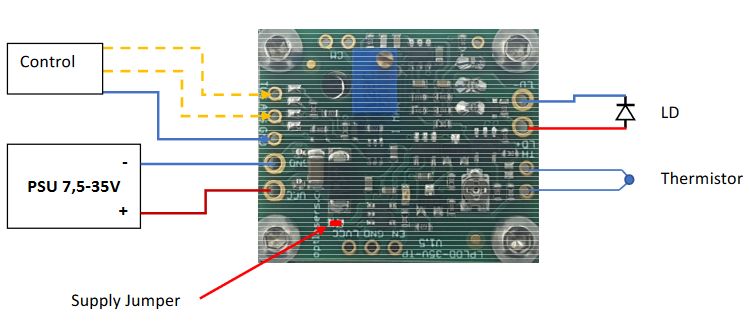
\includegraphics[scale=0.6, trim={0mm 0mm 0mm 0mm}, clip]{98_images/ldd_schema_connections.PNG}
    \caption{Das Schema des Diodentreibers von \textit{OptLaser} wie dieser mit den anderen Komponenten der Steuerung verbunden ist.}
    \label{fig:diodentreiber_schema_hw}
\end{figure}

Die in der Abb. \ref{fig:diodentreiber_modus_hw} gezeigte Darstellung ist das Signal zu ansteuern des Diodentreibers. Die dunkel blaue (unterste) Linie, ist das Ausgangssignal des Diodentreibers, das direkt in die Pumpdiode eingespeist wird. Die grüne (mittlere) Linie, ist das Signal am analogen Eingang des Diodentreibers. Damit wird die Stromstärke am Ausgang des Diodentreibers gesteuert. Die orange (oberste) Linie ist das \textit{Toggle}-Signal, dies gibt die Ansteuerung frei, damit das analoge Signal zum Ausgang des Diodentreibers gelangt.

\begin{figure}[H]
    \centering
    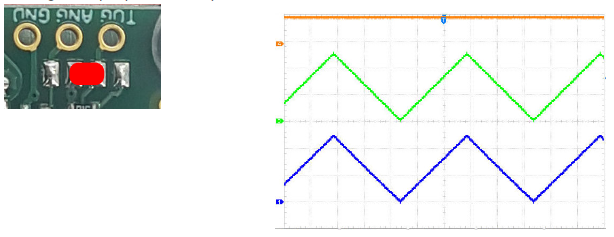
\includegraphics[scale=0.75, trim={70mm 0mm 0mm 0mm}, clip]{98_images/ldd_schema_modus.PNG}
    \caption{Die Steuerungssignale für den Diodentreiber von \textit{OptLaser}}
    \label{fig:diodentreiber_modus_hw}
\end{figure}

\subsection{Energieversorgung}
Die benötigte Leistung des Netzteils für das gesamte System beläuft sich auf etwa 80W. Dies wurde einerseits errechnet (s. Anhang \ref{formula:_calculation_sp_power}), andererseits mit einem Netzteil an dem alle Komponenten, bis auf den Diodentreiber angeschlossen wurden verifiziert. Die Pumpdiode wird mit 30V gespiesen, wohingegen der Rest der Steuerung mit 24V betrieben wird. Dies verlangte, dass entweder zwei Netzteile eingesetzt wurden oder aber ein Netzteil und ein DC/DC-Wandler, der die Spannung des Netzteils auf die benötigten 24V herunter regelt zum Einsatz kommt. Die Entscheidung viel auf einen DC/DC-Wandler, weil dieser im Volumen kleiner ist und somit weniger Platz im Gehäuse in Anspruch nimmt. Dieser kann eine Spannung von bis zu 36V aufnehmen und misst 24V beim Ausgang.

\begin{figure}[H]
%https://www.reichelt.com/ch/de/schaltnetzteil-geschlossen-195-w-36-v-5-5-a-mw-rsp-200-36-p147907.html?PROVID=2808&gad_source=1&gclid=Cj0KCQiA5-uuBhDzARIsAAa21T-__vZqX_esib7CfoGVmrPyoBO7UXEfQpRHOOkOo2j1YGIXCt2oLD0aAhbVEALw_wcB
    \centering
    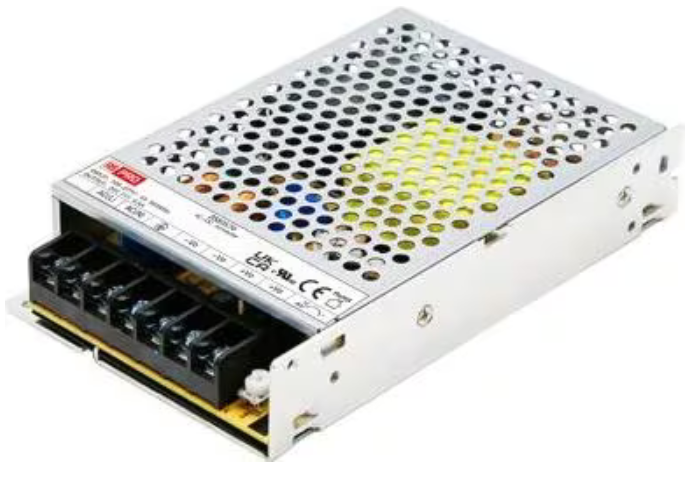
\includegraphics[scale=0.7]{98_images/controller_ps.PNG}
    \caption{Das Netzteil des Herstellers \textit{Mean Well}. [15]}
    \label{fig:controller_ps_hw}
\end{figure}

\begin{figure}[H]
% https://www.conrad.ch/de/p/mean-well-rsd-30g-24-dc-dc-wandler-12-v-dc-24-v-dc-36-v-dc-24-v-dc-1-25-a-30-w-1761269.html?gclid=CjwKCAiA6KWvBhAREiwAFPZM7vuk7TGgJgOWfGuP3-sRh1IH8ajzLsO8kXYmecqB9bC_QCBB2CDiuhoC8NAQAvD_BwE&utm_source=google-shopping-de&utm_medium=search&utm_campaign=shopping-online-de&utm_content=shopping-ad_cpc&WT.srch=1&ef_id=CjwKCAiA6KWvBhAREiwAFPZM7vuk7TGgJgOWfGuP3-sRh1IH8ajzLsO8kXYmecqB9bC_QCBB2CDiuhoC8NAQAvD_BwE%3AG%3As&gad_source=1
    \centering
    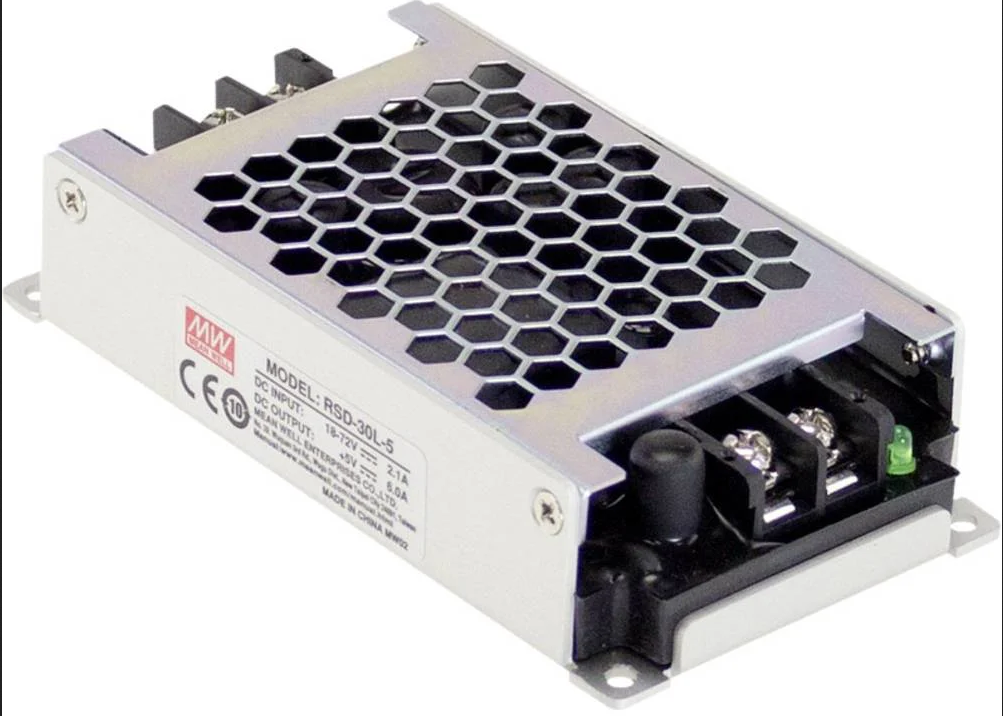
\includegraphics[scale=0.25, trim={1mm 1mm 1mm 1mm}, clip]{98_images/mean_well_dc_dc_converter.PNG}  
    \caption{Der eingesetzte DC/DC-Wandler, ebenfalls des Herstellers \textit{Mean Well}. [15]}
    \label{fig:dc_dc_wandler_hw}
\end{figure}

\subsection{Sensorik}
Die Positionen der Temperaturmessung des Alexandritkristalls und der Diode sind in Abbildung \ref{fig:temp_measurement_hw} dargestellt. An diesen Positionen stören sie den Laser im Betrieb nicht und können trotzdem die Temperatur möglichst nahe an der Quelle messen.\\

\begin{figure}[H]
    \centering
    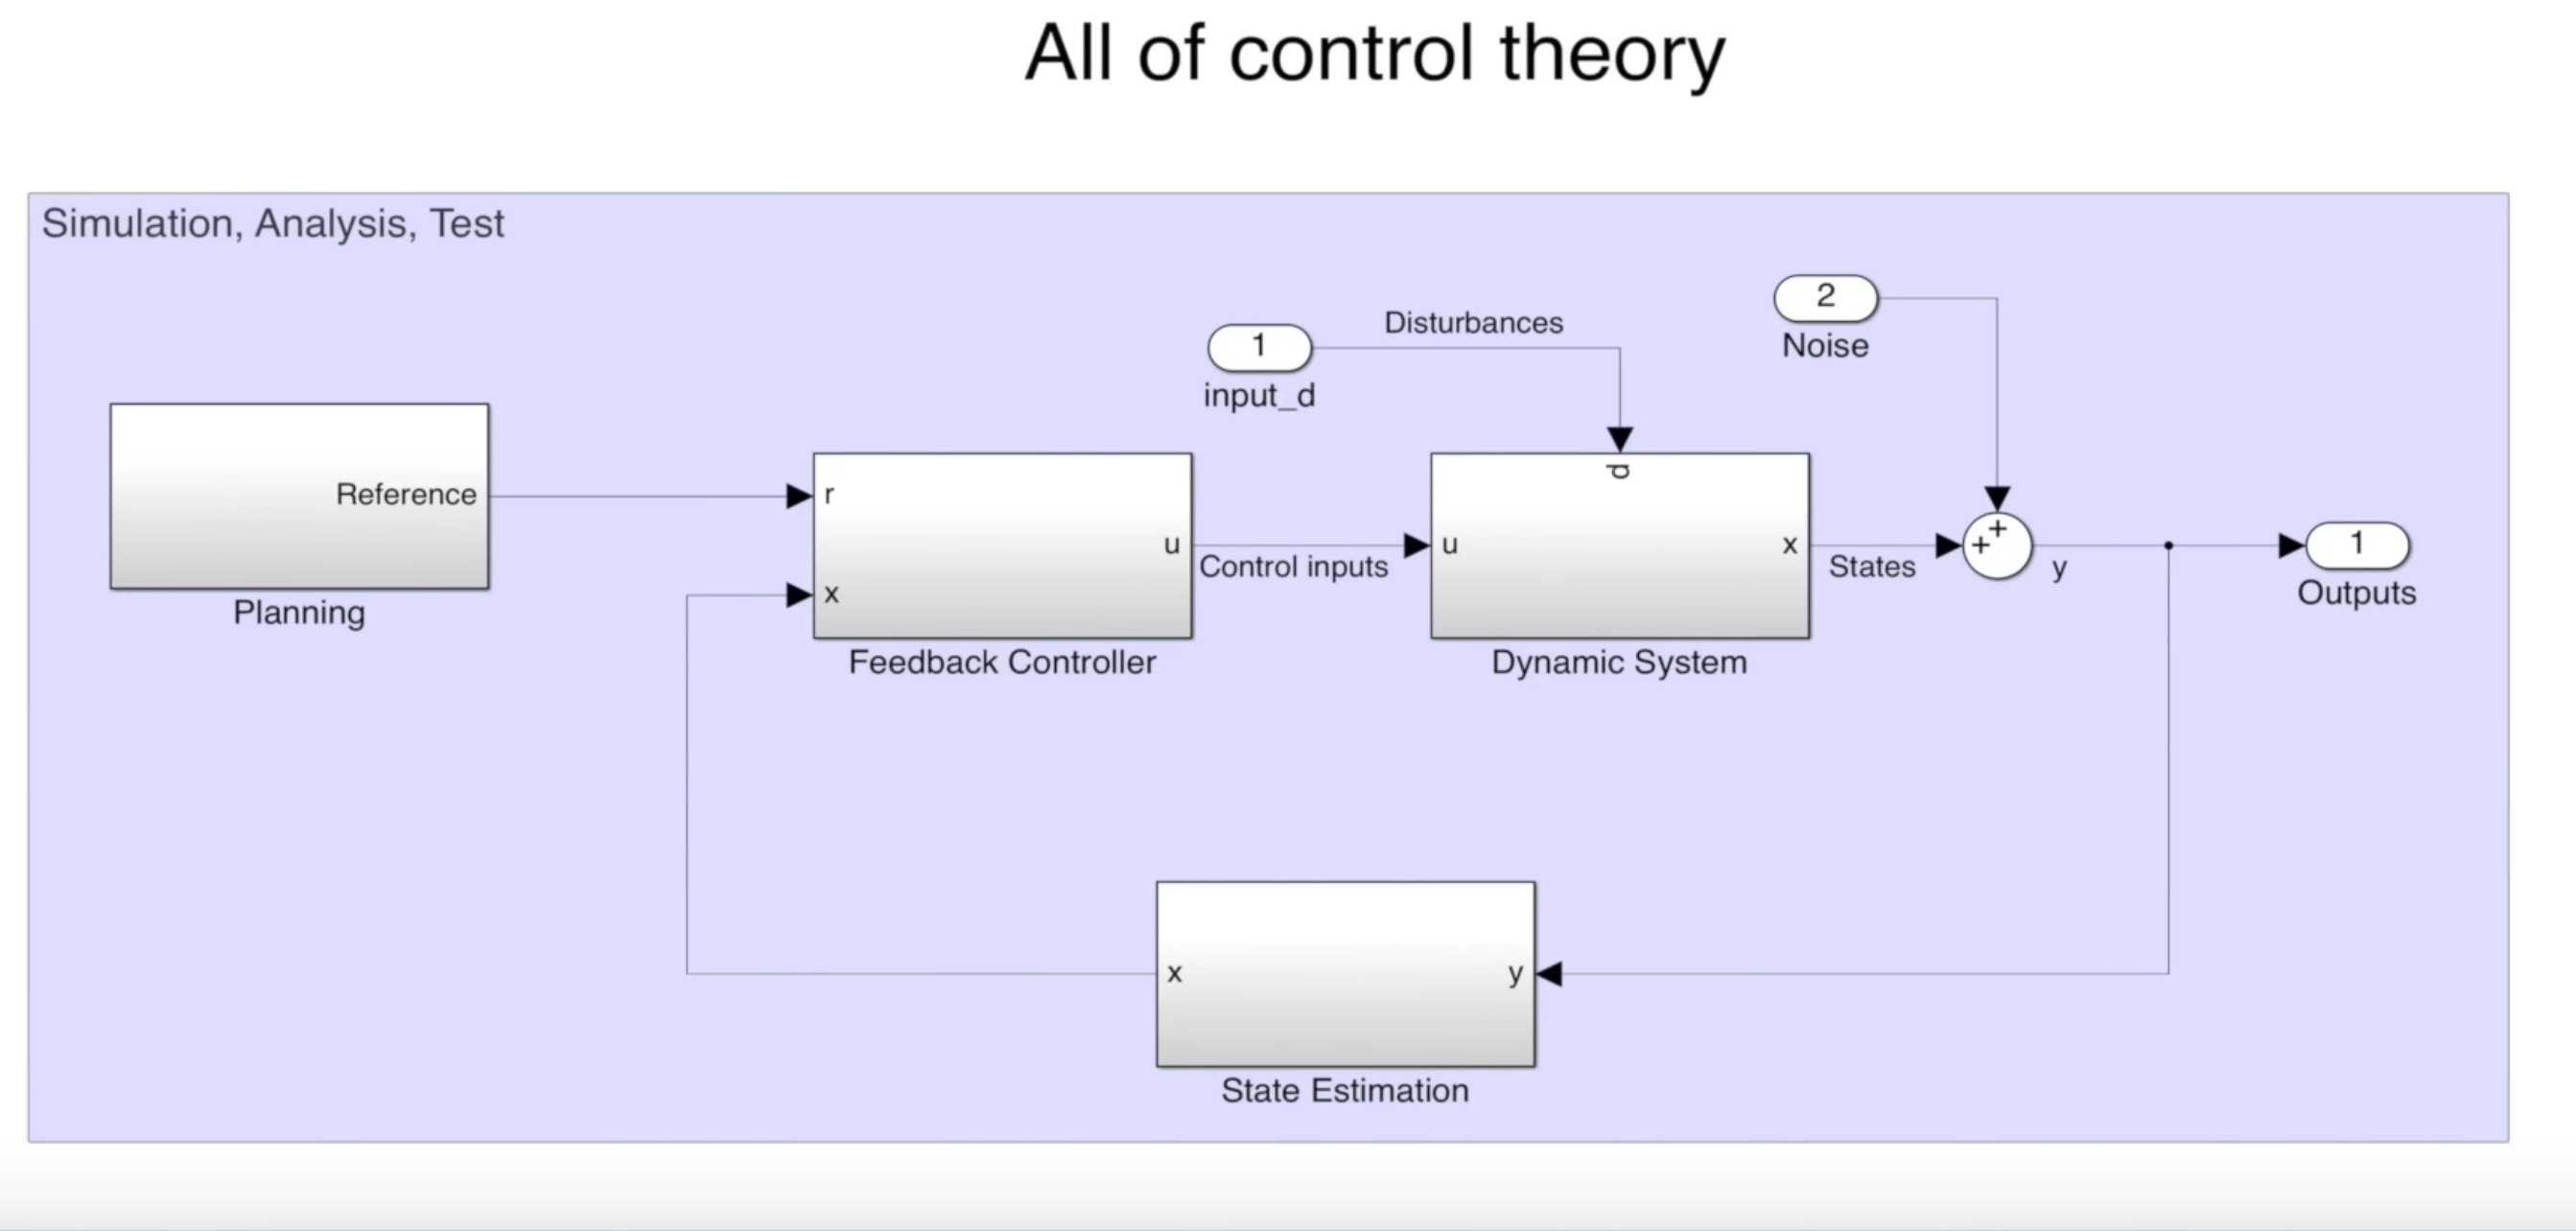
\includegraphics[scale=0.2]{98_images/all_control_theory.PNG}
    \caption{Positionen der Temperaturfühler für die Diode.}
    \label{fig:temp_measurement_hw}
\end{figure}

\begin{figure}[H]
    \centering
    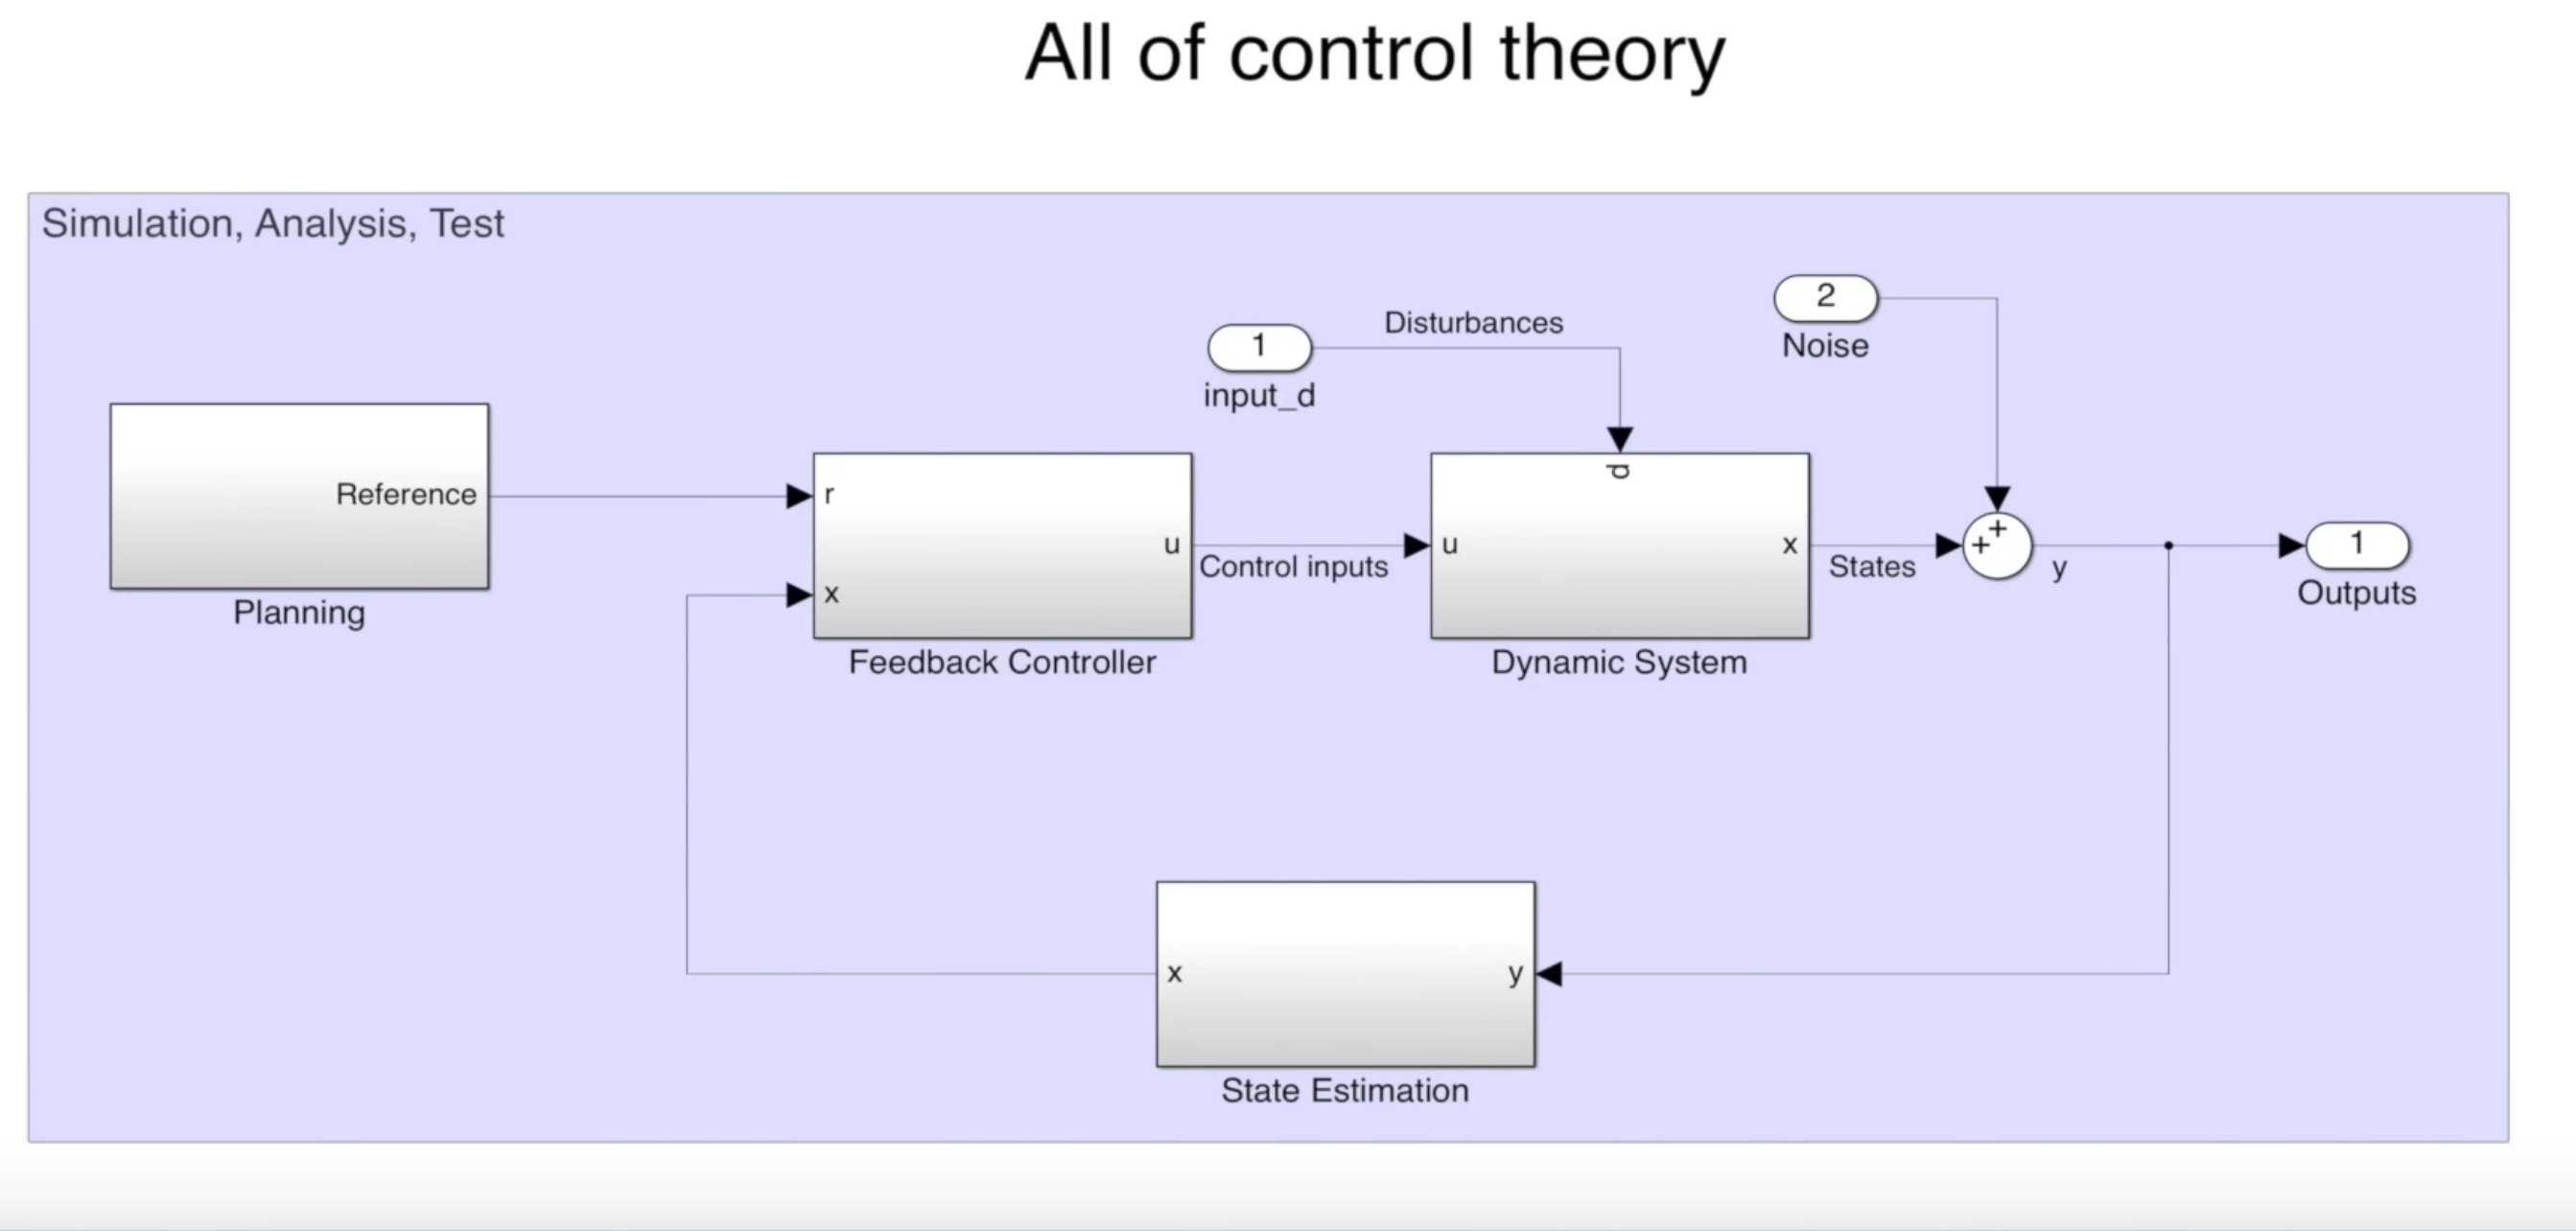
\includegraphics[scale=0.2]{98_images/all_control_theory.PNG}
    \caption{Positionen der Temperaturfühler für den Kristall.}
    \label{fig:temp_measurement_hw}
\end{figure}
% \subsection{Verkabelung}  % Architektur der Verkabelung
% Die externe Verkabelung des Gehäuses bzw. dessen Komponenten, soll mit einem \textbf{XYZ}-Kabel erfolgen. Somit können alle Komponente, die zum Laser gehen kompakt in einem Kabel geführt werden.\\
% Intern werden die Komponente mit einem \textbf{XYZ}-Kabel verdrahtet und werden über einen Kabelbaum geführt.\textbf{NICHT NÖTIG!!!!!!!!!!}\\
% 
% \begin{figure}[H]
%     \centering
%     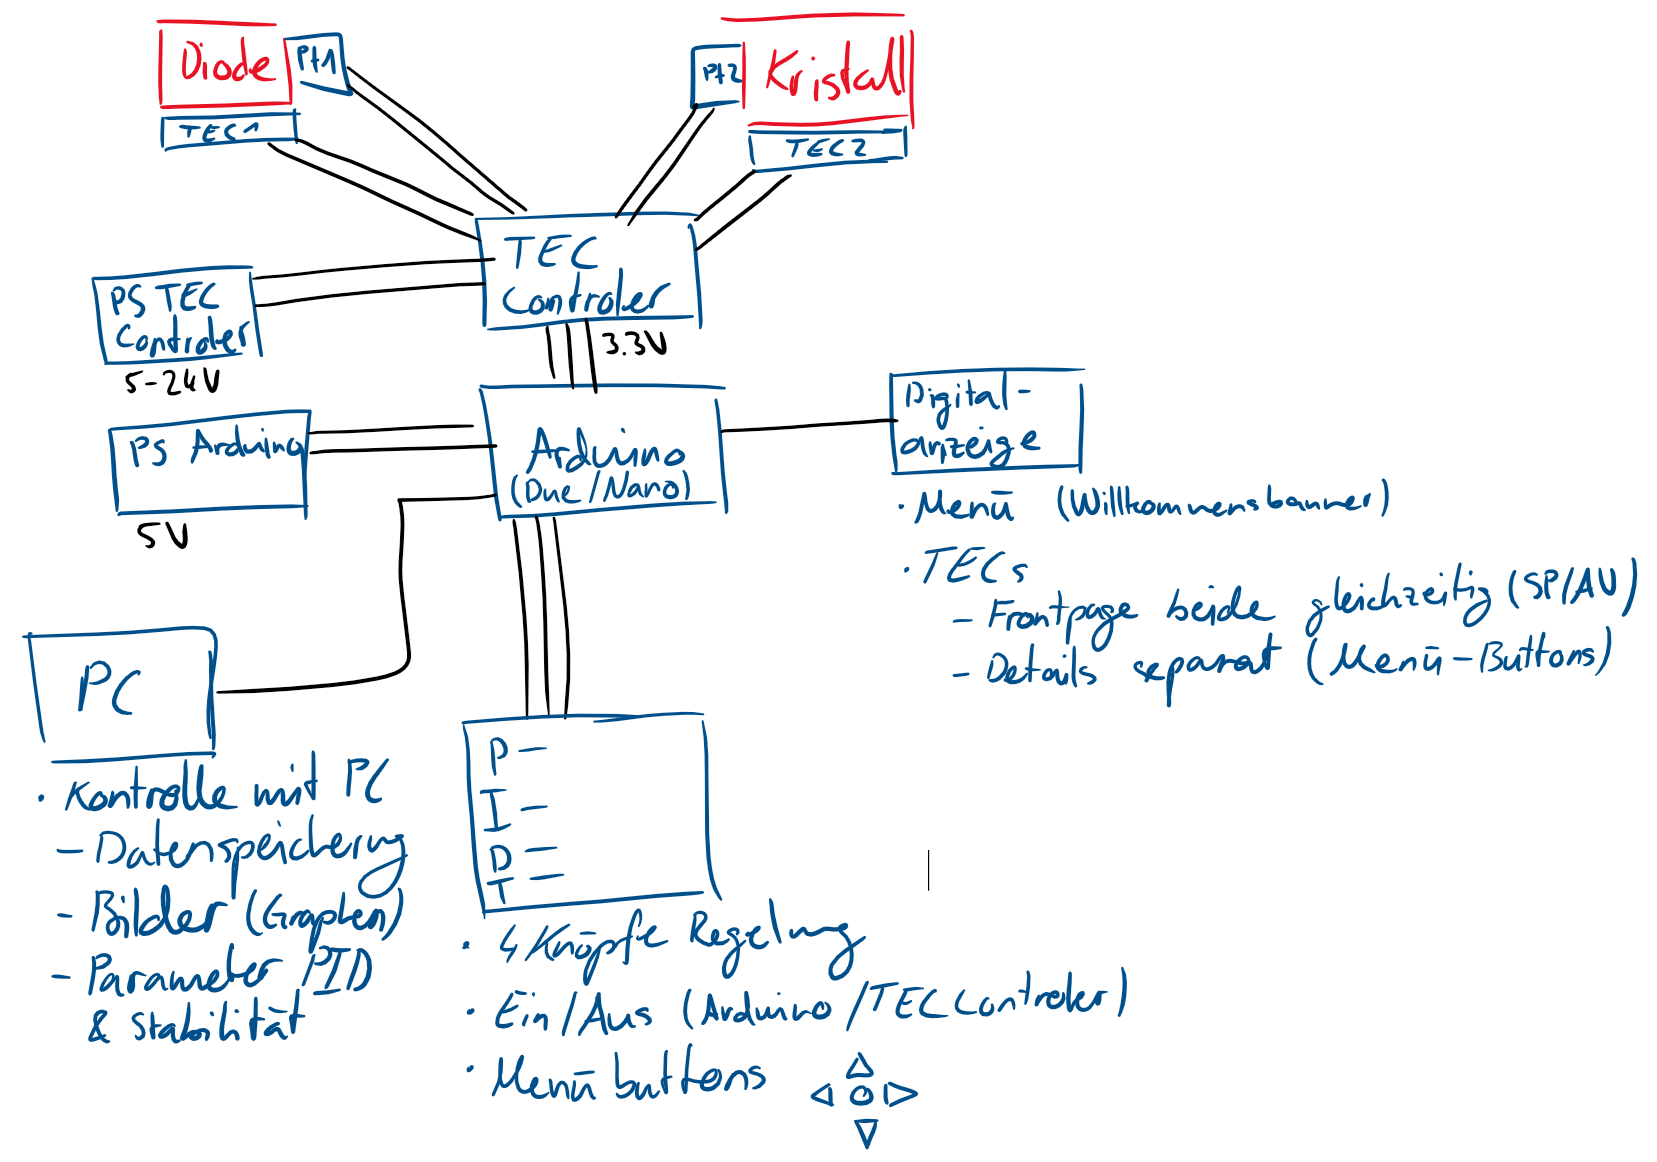
\includegraphics[scale=0.5]{98_images/scheme_wiring.PNG}
%     \caption{Verkabelung der elektrischen Komponenten.}
%     \label{fig:scheme_wiring_hw}
% \end{figure}

\subsection{Die Digitalanzeige}
Für die Digitalanzeige waren vor allem drei Aspekte ausschlaggebend, um die gewünschte Funktion zu gewährleisten. Die Eingabe der Werte, die Anzeige der Werte und Verständlichkeit der angezeigten Werte. All die Kriterien sollten erfüllt werden, um die Steuerung des Lasers optimal zu gewährleisten. In der Folgenden Tabelle wurden einige Kriterien, die die zuvor genannten Aspekte ermöglichen sollen. Auch aus Sicherheitsgründen muss die Ergonomie der Anzeige intuitiv gestaltet sein und muss im Notfall handhabbar bleiben. Es werden zwei Displaytypen einander gegenüber gestellt.

\begin{table}[H]
    \centering
    \begin{tabular}{l|l|l}
        \multicolumn{1}{c|}{$-$}&        \textbf{16x2 mit Taster}&       \textbf{800x480 Touchanzeige}\\
        \hline
        Bedienung&                      $-$ Taster Analogeingänge&      $+$ Touch integriert\\
        Anzeige&                        $-$ Kleine Anzeige&             $+$ Grössere Anzeige\\
        Verständlichkeit&               $-$ Kryptische Anzeige&         $+$ Verständliche Anzeige\\
        Benutzerführung&                 $-$ Tieferes Menü&              $+$ Weniger tiefes Menü\\
        Programmierung&                 $+$ Einfache Programmierung&    $-$ Anspruchsvolle Programmierung
    \end{tabular}
    \caption{Pro - Kontra Liste für die Auswahl der Digitalanzeige}
    \label{tab:choice_display_hw}
\end{table}

Die Entscheidung fiel auf die Touchanzeige. Zusätzlich lassen sich alle Komponente wie Knöpfe direkt in die Anzeige programmieren. Es müssen keine komplexen Abläufe programmiert werden, die die Betätigung der physischen Knöpfe erkennt und das Programm lenkt. Zusätzlich müssen keine Ein-/Ausgänge zusätzlich auf der SPS einprogrammiert werden. Mit der Anzeige können ganze Designs erstellt werden, was das Arbeiten mit der Steuerung ergonomischer macht.

\subsection{Konstruktion des Gehäuses}
Das Gehäuse war bereits vorhanden. Die oben aufgelisteten Komponenten wurden auf zusätzlichen Blechen montiert, in die Gewindelöcher eingebracht wurden. Durch die konvexe Form der Seiten des Gehäuses entstand im Inneren des Kontrollers mehr Fläche für die Komponenten und vereinfachte dadurch die Montage. Zusätzlich mussten noch die Zugänge für die Verkabelung der Stromversorgung, deren Schalter und das Kabel für die Ansteuerung der Komponenten im Laser-Aufbau angepasst werden. Dafür wurden sämtliche Löcher für spätere Erweiterungen beibehalten.

\begin{figure}[H]
    \centering
    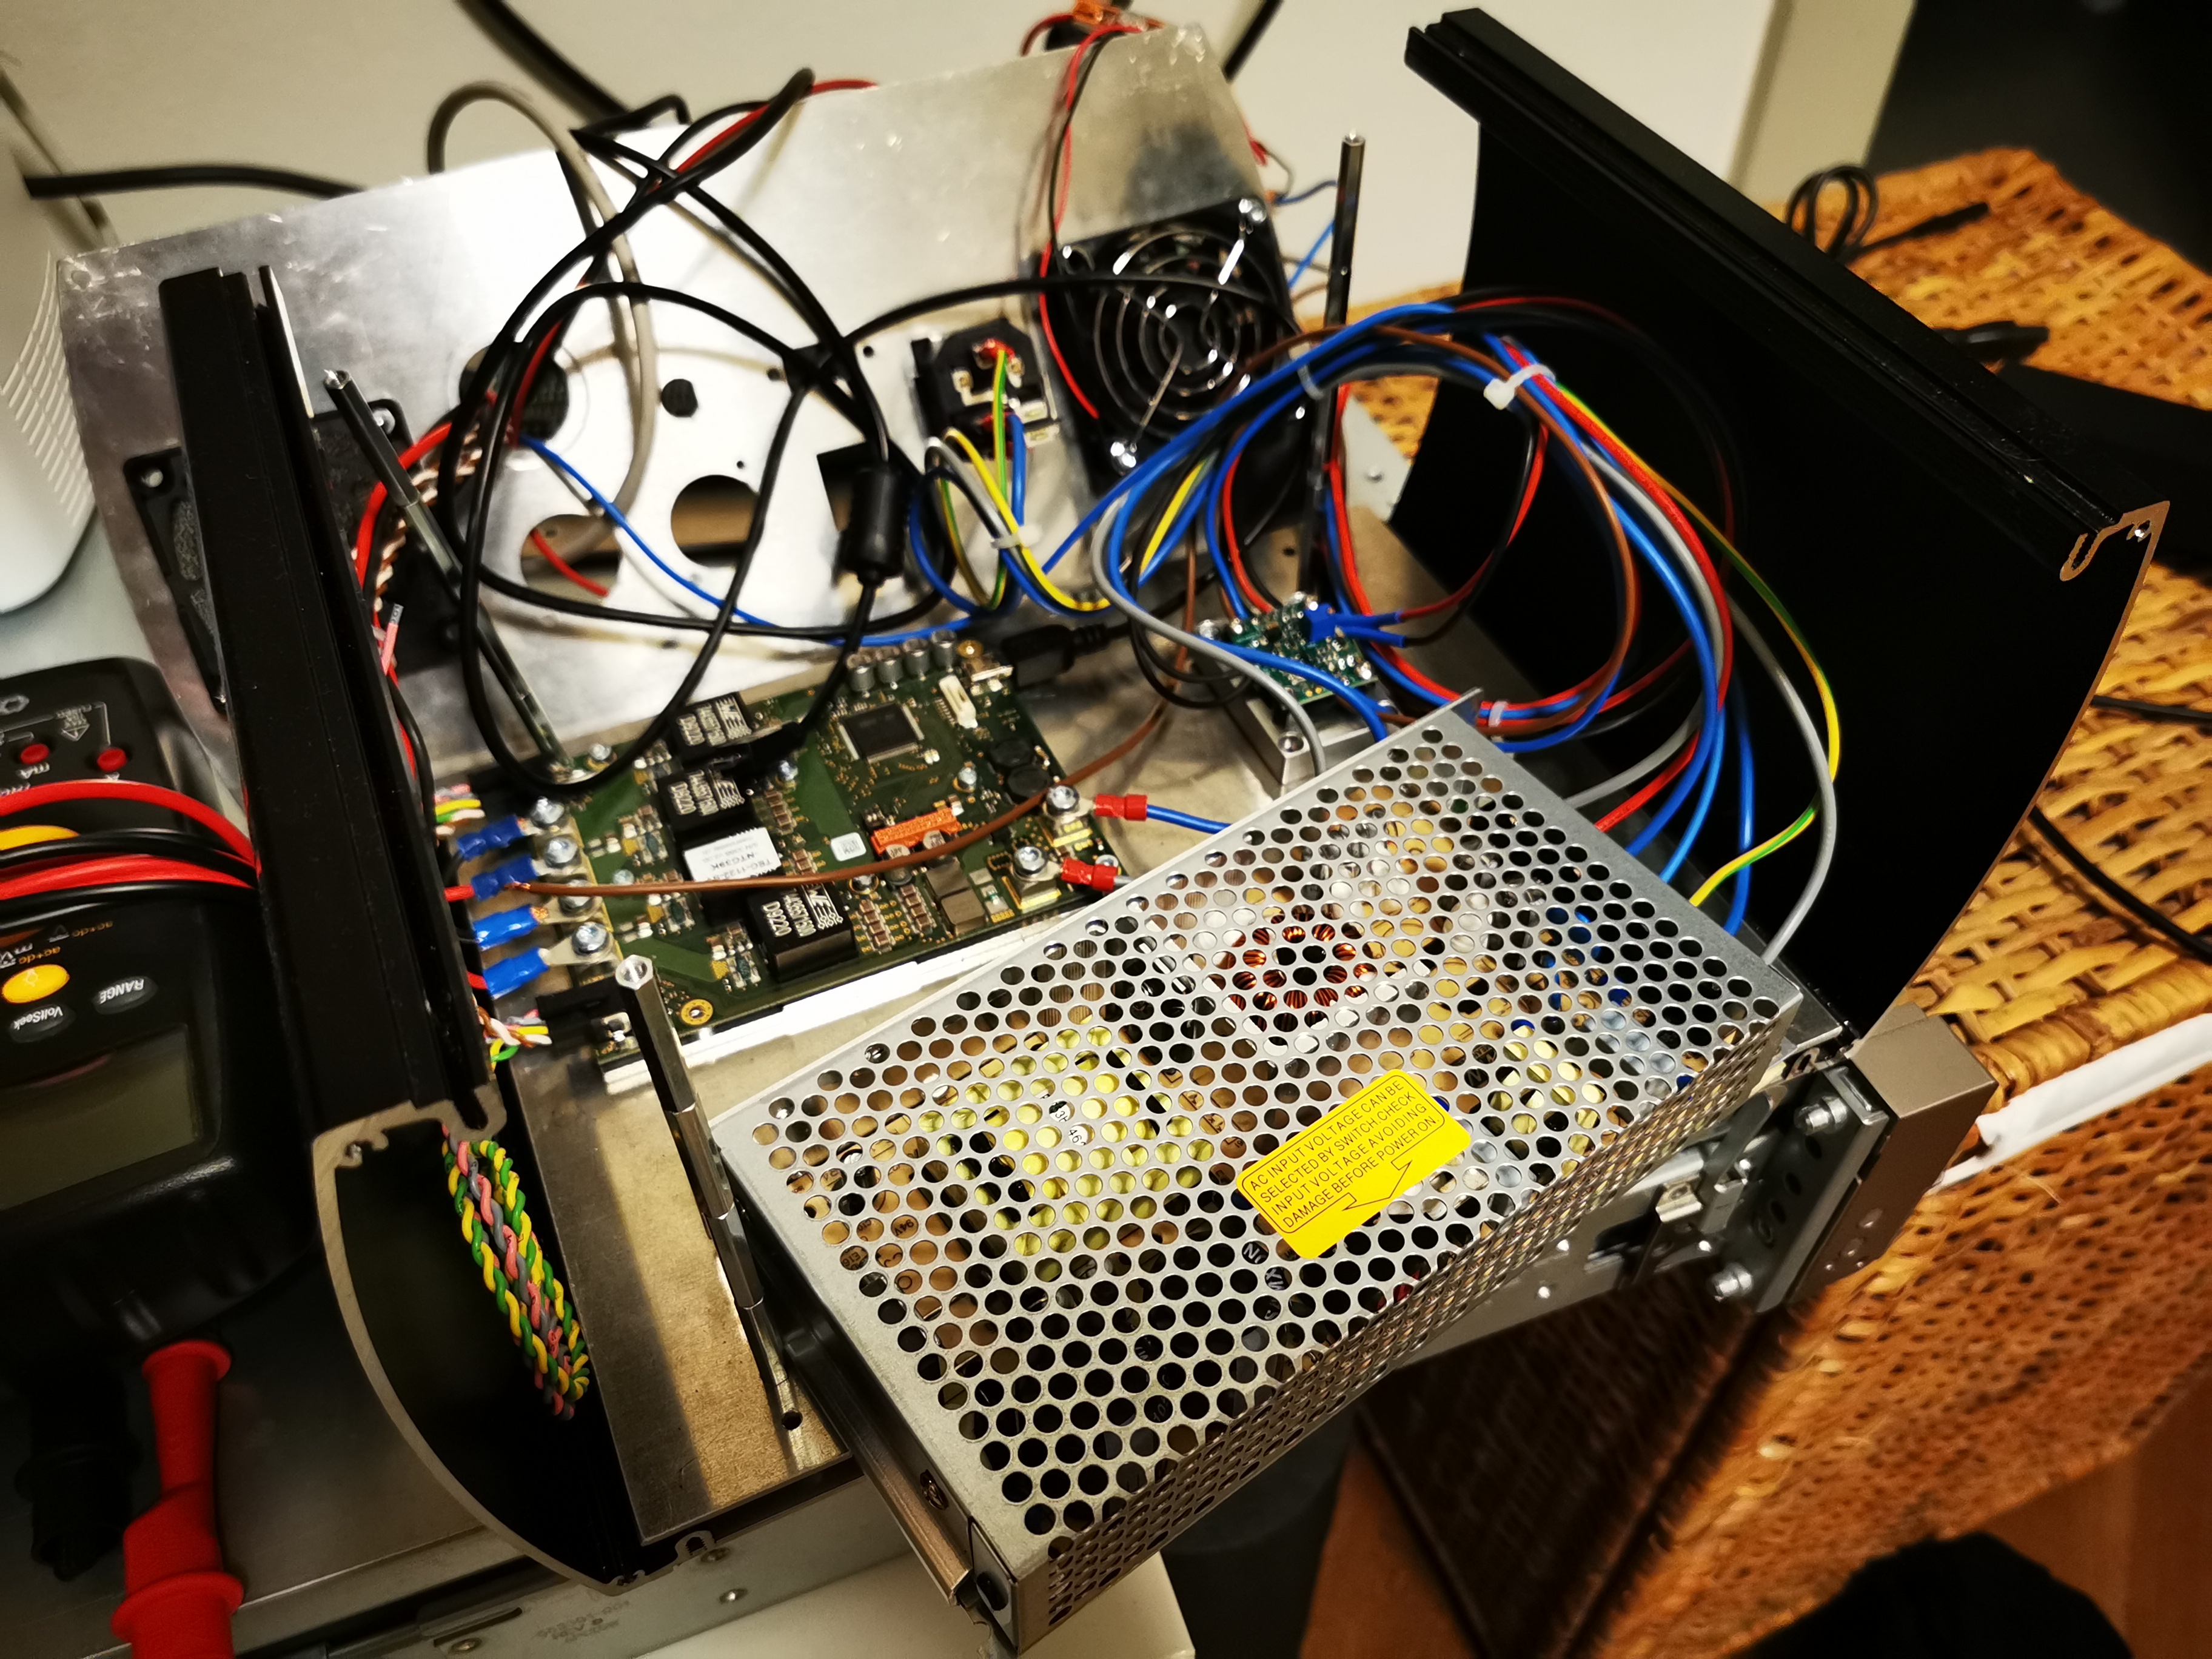
\includegraphics[scale=0.08]{98_images/housing_inside.jpg}
    \caption{Das Innenleben der Steuerung.}
    \label{fig:enter-label}
\end{figure}
\subsection{Testaufbau - Mock-up}
In einem Mock-up konnten die Funktionen und das Verhalten der Steuerung geprüft werden. Darunter wurde getestet, ob die Temperaturen in der Steuerung in einem gewünschten Rahmen von 40°C-65°C blieben. $[13]$ Zur Referenz wurde die interne Messung der CPU verwendet. Gemessen werden die Temperaturen mit der internen Temperaturmessung des Prozessors des Raspberry PI. Die Temperatur im Gehäuse wurde dann von der Temperatur des Prozessors abgeleitet. Dafür wurde sie mit einem Temperaturmessgerät extern gemessen und die Messergebnisse mit denen des Prozessors verknüpft.
Die Positionen der Komponenten im Gehäuse wurde mit Hilfe von CAD-Software geprüft. Danach wurden die oben genannten Bleche erstellt und die Komponente mit Verschraubungen platziert.